\section{RRTSlide  Class Reference}
\label{class_RRTSlide}\index{RRTSlide@{RRTSlide}}
In the Connect method, slide along the walls. 


{\tt \#include $<$rrtslide.h$>$}

Inheritance diagram for RRTSlide::\begin{figure}[H]
\begin{center}
\leavevmode
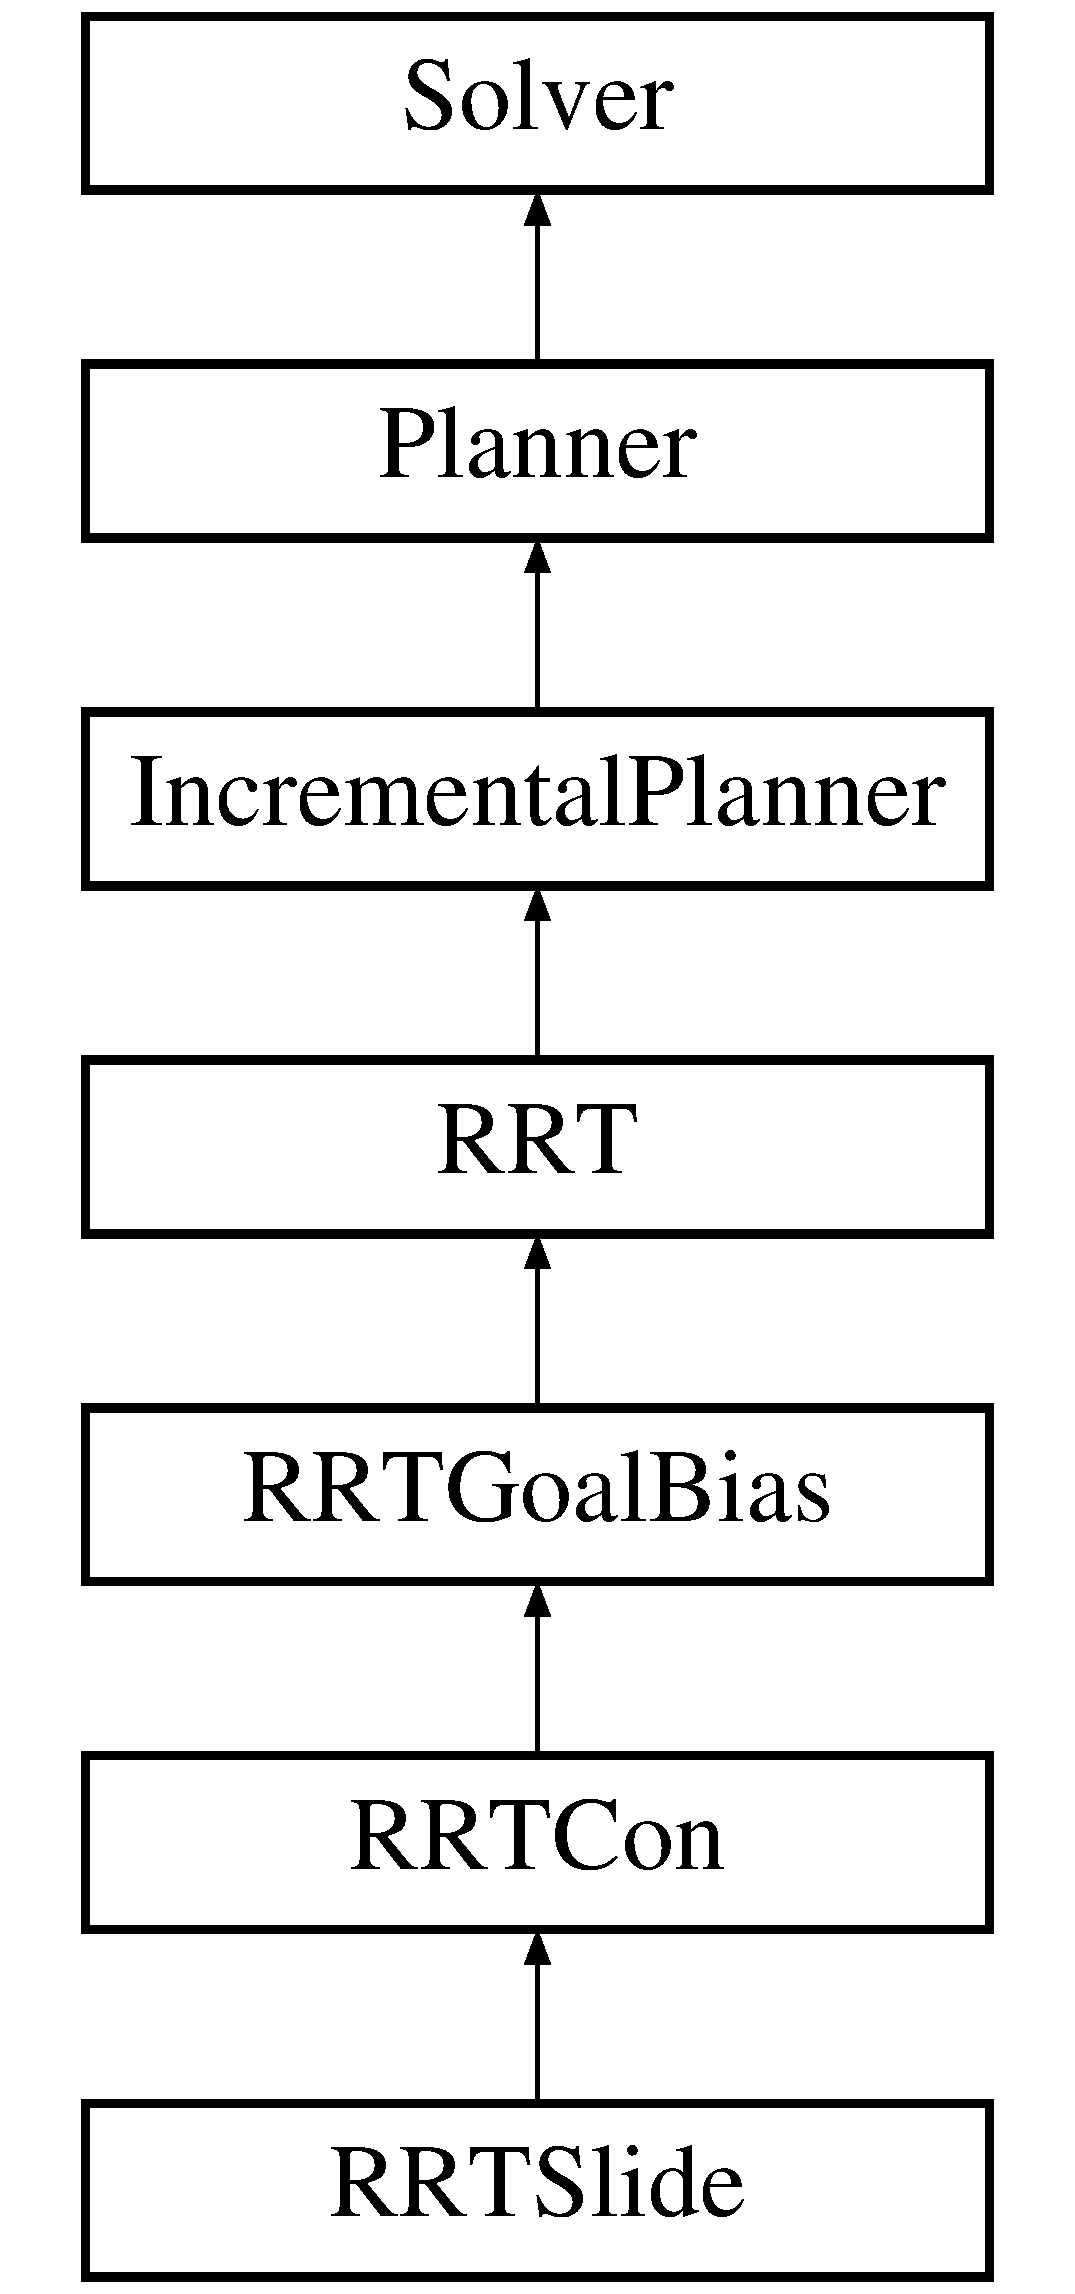
\includegraphics[height=7cm]{class_RRTSlide}
\end{center}
\end{figure}
\subsection*{Public Methods}
\begin{CompactItemize}
\item 
{\bf RRTSlide} ({\bf Problem} $\ast$p)
\item 
virtual {\bf $\sim$RRTSlide} ()
\item 
virtual {\bf MSLVector} {\bf Select\-Input} (const {\bf MSLVector} \&x1, const {\bf MSLVector} \&x2, {\bf MSLVector} \&nx\_\-best, bool \&success, bool forward)
\begin{CompactList}\small\item\em Select the input that gets closest to x2 from x1.\item\end{CompactList}\item 
virtual bool {\bf Connect} (const {\bf MSLVector} \&x, {\bf MSLTree} $\ast$t, {\bf MSLNode} $\ast$\&nn, bool forward)
\begin{CompactList}\small\item\em Iterated Extend.\item\end{CompactList}\item 
{\bf MSLVector} {\bf Random\-Direction} ()
\end{CompactItemize}
\subsection*{Public Attributes}
\begin{CompactItemize}
\item 
int {\bf Random\-Trials}
\item 
int {\bf Num\-Directions}
\item 
vector$<${\bf MSLVector}$>$ {\bf Random\-Directions}
\end{CompactItemize}


\subsection{Detailed Description}
In the Connect method, slide along the walls.



\subsection{Constructor \& Destructor Documentation}
\index{RRTSlide@{RRTSlide}!RRTSlide@{RRTSlide}}
\index{RRTSlide@{RRTSlide}!RRTSlide@{RRTSlide}}
\subsubsection{\setlength{\rightskip}{0pt plus 5cm}RRTSlide::RRTSlide ({\bf Problem} $\ast$ {\em p})}\label{class_RRTSlide_a0}


\index{RRTSlide@{RRTSlide}!~RRTSlide@{$\sim$RRTSlide}}
\index{~RRTSlide@{$\sim$RRTSlide}!RRTSlide@{RRTSlide}}
\subsubsection{\setlength{\rightskip}{0pt plus 5cm}RRTSlide::$\sim$RRTSlide ()\hspace{0.3cm}{\tt  [inline, virtual]}}\label{class_RRTSlide_a1}




\subsection{Member Function Documentation}
\index{RRTSlide@{RRTSlide}!Connect@{Connect}}
\index{Connect@{Connect}!RRTSlide@{RRTSlide}}
\subsubsection{\setlength{\rightskip}{0pt plus 5cm}bool RRTSlide::Connect (const {\bf MSLVector} \& {\em x}, {\bf MSLTree} $\ast$ {\em t}, {\bf MSLNode} $\ast$\& {\em nn}, bool {\em forward})\hspace{0.3cm}{\tt  [virtual]}}\label{class_RRTSlide_a3}


Iterated Extend.



Reimplemented from {\bf RRT} {\rm (p.\,\pageref{class_RRT_b3})}.\index{RRTSlide@{RRTSlide}!RandomDirection@{RandomDirection}}
\index{RandomDirection@{RandomDirection}!RRTSlide@{RRTSlide}}
\subsubsection{\setlength{\rightskip}{0pt plus 5cm}{\bf MSLVector} RRTSlide::Random\-Direction ()}\label{class_RRTSlide_a4}


\index{RRTSlide@{RRTSlide}!SelectInput@{SelectInput}}
\index{SelectInput@{SelectInput}!RRTSlide@{RRTSlide}}
\subsubsection{\setlength{\rightskip}{0pt plus 5cm}{\bf MSLVector} RRTSlide::Select\-Input (const {\bf MSLVector} \& {\em x1}, const {\bf MSLVector} \& {\em x2}, {\bf MSLVector} \& {\em nx\_\-best}, bool \& {\em success}, bool {\em forward})\hspace{0.3cm}{\tt  [virtual]}}\label{class_RRTSlide_a2}


Select the input that gets closest to x2 from x1.



Reimplemented from {\bf RRT} {\rm (p.\,\pageref{class_RRT_b0})}.

\subsection{Member Data Documentation}
\index{RRTSlide@{RRTSlide}!NumDirections@{NumDirections}}
\index{NumDirections@{NumDirections}!RRTSlide@{RRTSlide}}
\subsubsection{\setlength{\rightskip}{0pt plus 5cm}int RRTSlide::Num\-Directions}\label{class_RRTSlide_m1}


\index{RRTSlide@{RRTSlide}!RandomDirections@{RandomDirections}}
\index{RandomDirections@{RandomDirections}!RRTSlide@{RRTSlide}}
\subsubsection{\setlength{\rightskip}{0pt plus 5cm}vector$<${\bf MSLVector}$>$ RRTSlide::Random\-Directions}\label{class_RRTSlide_m2}


\index{RRTSlide@{RRTSlide}!RandomTrials@{RandomTrials}}
\index{RandomTrials@{RandomTrials}!RRTSlide@{RRTSlide}}
\subsubsection{\setlength{\rightskip}{0pt plus 5cm}int RRTSlide::Random\-Trials}\label{class_RRTSlide_m0}




The documentation for this class was generated from the following file:\begin{CompactItemize}
\item 
{\bf rrtslide.h}\end{CompactItemize}
